\documentclass[a4paper,11pt]{article}
\usepackage[T1]{fontenc}
\usepackage[utf8]{inputenc}
\usepackage[spanish]{babel}
\usepackage{listings}
\usepackage{hyperref}
\usepackage{graphicx}
\usepackage{titling}

\usepackage{fancyhdr}

\pagestyle{fancy}
\fancyhf{} 

\lhead{
\includegraphics[width=2cm]{logo-unsa}}
\chead{Universidad Nacional de San Agustín}
\rhead{\thepage}

\lfoot{Instituto Astronómico Aeroespacial Pedro Paulet}
\rfoot{
\includegraphics[width=3cm]{logo-iaapp}}

\renewcommand{\headrulewidth}{0.5pt}
\renewcommand{\footrulewidth}{0.5pt}

\lstset
{
    basicstyle=\ttfamily,
    basicstyle=\footnotesize,
    columns=fullflexible,
    frame=single,
    breaklines=true,
%     xleftmargin=0cm,
%   xrightmargin=0cm,
    aboveskip=0.5cm,
    belowskip=0.2cm,
%   frame=tlbr,
%   framesep=0pt,
%   showspaces=false,                          % show spaces (with underscores)
    resetmargins=true, 
    postbreak=\kern-4.5ex
%   framerule=1pt, 
%   numbers=left
%   postbreak=\mbox{\textcolor{red}{$\hookrightarrow$}\space},
}

\setlength{\columnsep}{0.8cm}
% \renewcommand*\sectionformat{\thesection\autodot\hspace{0.2cm}}

\makeatletter
\renewcommand*{\@seccntformat}[1]{\csname the#1\endcsname\hspace{0.4cm}}
\makeatother

%opening
\title{Manual de uso de Inkari}
\author{Ronald Darwin Apaza Veliz}

\graphicspath{ {images/} }

\newenvironment{note}
{
    \vspace{0.22cm}
    \noindent
    \textbf{Nota: }
}
{
    \vspace{0.22cm}
}

\begin{document}

\begin{titlepage}
	\centering
    \vspace*{0.5 cm}
    
\includegraphics[scale = 0.55]{logo-inkari}\\[1.0 cm]	% University Logo
    \textsc{\LARGE \newline\newline Supercomputadora Inkari}\\[2.0 cm]	% University Name
	\textsc{\Large Universidad Nacional de San Agustín}\\[0.5 cm]				% Course Code
	\rule{\linewidth}{0.2 mm} \\[0.4 cm]
	{ \huge \bfseries \thetitle}\\
	\rule{\linewidth}{0.2 mm} \\[1.5 cm]
	
	\begin{minipage}{0.5\textwidth}
		\begin{flushleft}
            \large
			\emph{Autor:}\\
			Ronald Apaza
        \end{flushleft}
        \end{minipage}
        ~
        \begin{minipage}{0.4\textwidth}    
			\begin{flushright}
                \large
                \emph{Grupo:} \\
                IAAPP
            \end{flushright}
	\end{minipage}\\[2 cm]
	
    \today

\end{titlepage}

% \twocolumn
% \sloopy

\section{Introducción}

En el ámbito de la computación nos referimos como clúster a un conjunto de ordenadores conectados entre sí y que mediante un software específico permite realizar operaciones de forma simultánea, proporcionado así, una mayor capacidad de cómputo.

\section{Conexión al clúster}

Para conectarse al clúster es necesario disponer previamente de una cuenta. Para solicitar una cuenta, se debe de escribir un correo electrónico a: inkari.unsa@gmail.com.

\subsection{Acceso desde Linux}

La mayoría de los ordenadores con Linux vienen dotadas de un cliente ssh que puede ser invocado directamente desde el terminal mediante el siguiente comando:

\begin{lstlisting}
ssh <cuenta>@inkari.unsa.edu.pe
\end{lstlisting}

\subsection{Acceso desde Windows}

Para acceder al clúster en windows será necesario utilizar un cliente ssh. Putty es uno de los clientes más populares y ligeros, este puede ser descargado de: \url{http://www.chiark.greenend.org.uk/~sgtatham/putty/download.html}.
Una vez instalado, Putty nos ofrece la interfaz, mostrada en la figura \ref{fig:putty_1}:

\begin{figure}[!ht]
    \centering
    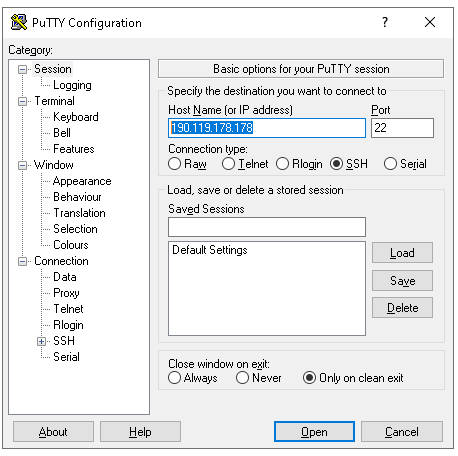
\includegraphics[width=6.2cm]{putty_1}
    \caption{Interfaz de inicio del programa Putty}
    \label{fig:putty_1}
\end{figure}

Tras colocar \textbf{inkari.unsa.edu.pe} (o su IP: inkari.unsa.edu.pe) en el campo Host Name, nos conectamos presionando el botón Open. Si es la primera vez que nos conectamos al clúster, se debe aceptar la alerta, mostrada en la figura \ref{fig:putty_alerta}:

\begin{figure}[!ht]
    \centering
    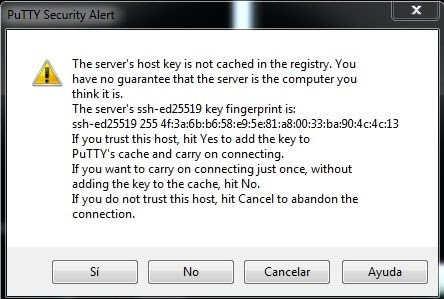
\includegraphics[width=8cm]{putty_alerta}
    \caption{Alerta mostrada por Putty, que solicita agregar el host como una fuente}
    \label{fig:putty_alerta}
\end{figure}

A continuación el cliente ssh, abrirá una terminal, en la cual se debe de introducir el usuario y la contraseña proporcionada por el administrador.

\begin{figure}[!ht]
    \centering
    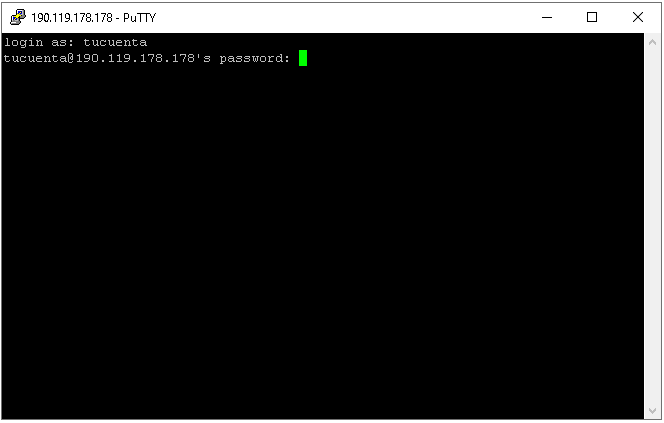
\includegraphics[width=10.5cm]{putty_terminal}
    \caption{Cliente SSH, solicitando los datos de acceso}
\end{figure}

\section{Primer acceso}

Si es la primera vez que se accede al clúster, será necesario cambiar la contraseña, para ello, tras iniciar sesión, se deberá colocar nuevamente la contraseña proporcionada por el administrador.

\begin{figure}[!ht]
    \centering
    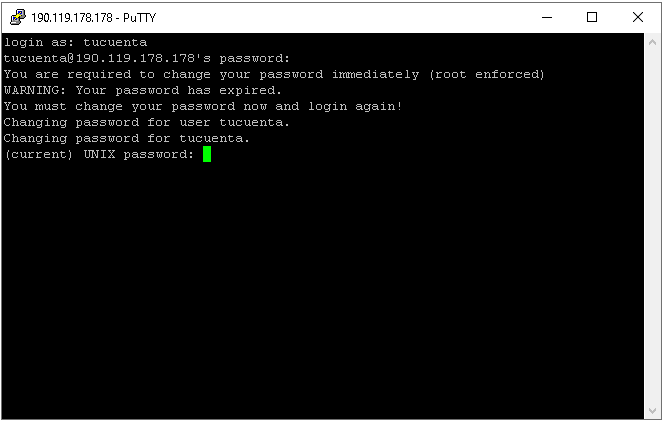
\includegraphics[width=10.5cm]{ssh_conf_old}
    \caption{Cliente SSH, solicitando que se confirme la contraseña asignada por el administrador}
\end{figure}

Y a continuación se deberá asignar una nueva contraseña, la cual debe de contener 2 números y al menos una letra en mayúscula.

\begin{figure}[!ht]
    \centering
    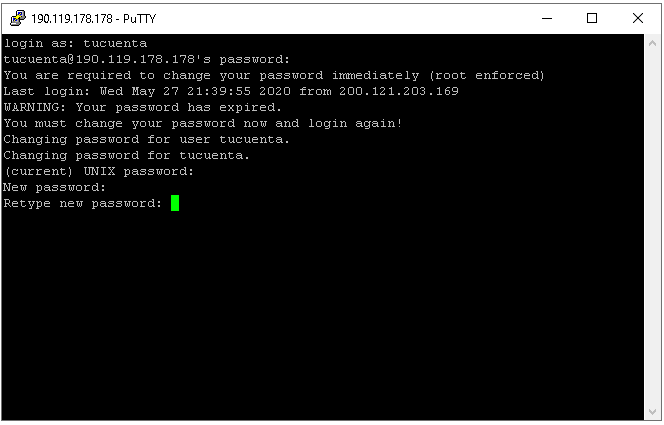
\includegraphics[width=10.5cm]{ssh_nueva_pass}
    \caption{Cliente SSH, solicitando una nueva contraseña}
\end{figure}

Una vez cambiada la contraseña, la sesión iniciada finalizará.

\section{Problemas de acceso}

Si tiene problemas para acceder a Inkari, una posibilidad es que ud. haya ingresado de manera \textbf{recurrente} una contraseña equivocada y ante ello Inkari haya baneado su IP al detectar dicha acción como una operación sospechosa, en caso de que su IP haya sido baneada, ud visualizará el siguiente mensaje: ``Conexión rehusada'' (tal y como en la figura \ref{fig:refused}).

\begin{figure}[!ht]
    \centering
    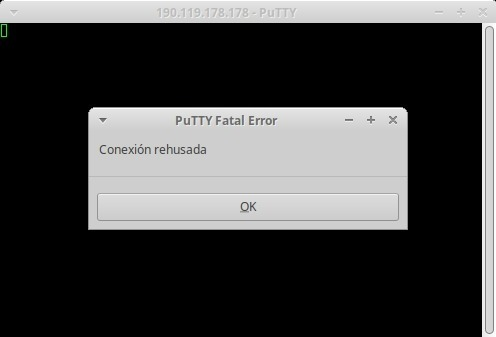
\includegraphics[width=7.5cm]{refused}
    \caption{Conexión SSH rechazada en Putty (posiblemente a causa de una IP baneada)}
    \label{fig:refused}
\end{figure}

En caso de que crea que su IP ue baneada, ud deberá de enviar un correo a la administración (inkari@unsa.edu.pe), indicando su dirección IP \textbf{pública}.

\begin{figure}[!ht]
    \centering
    
\includegraphics[width=10.5cm]{google}
    \caption{Conexión SSH rechazada en Putty (posiblemente a causa de una IP baneada)}
    \label{fig:google}
\end{figure}

Una forma de saber cuál es su IP pública es realizando una búsqueda en google con los siguientes términos: ``\textit{what is my ip}'', tal y como se muestra en la imagen \ref{fig:google}.

\section{Transferencia de archivos}

Para la ejecución de un job en Inkari, será necesario que copie todos los ficheros necesarios al clúster, es importante resaltar que todos los archivos almacenados en el clúster no serán respaldados por la administración de Inkari, motivo por el cual se recomienda a los usuarios, tomen las medidas de precaución correspondientes para sus archivos importantes.
Los usuarios solo pueden utilizar como almacenamiento de sus archivos sus respectivos espacios de trabajo, el espacio de trabajo de cada usuario puede ser accedido mediante la siguiente ruta absoluta:

\begin{center} 
    /home/<cuenta>
\end{center} 

También podrá acceder al espacio de trabajo utilizando la variable de entorno \$HOME.

\subsection{Transferencia de archivos desde Linux}

Para copiar archivos desde una computadora local al clúster, se puede utilizar el comando scp; a continuación se presenta el uso de este comando para subir un archivo al clúster.

\begin{lstlisting}
scp <ruta_del_archivo> <cuenta>@inkari.unsa.edu.pe:<ruta_del_destino>
\end{lstlisting}

En caso de que se desee descargar un archivo del clúster, el comando a utilizar es el siguiente:

\begin{lstlisting}
scp <cuenta>@inkari.unsa.edu.pe:<ruta_del_archivo> <ruta_del_destino>
\end{lstlisting}

Si se desea transferir carpetas en lugar de ficheros, se debe de agregar la bandera -r al comando scp. Por otra parte se recuerda al usuario que solo está permitida la transferencia de archivos menores a 200 megabytes.

\subsection{Transferencia de archivos desde Windows}

Una de las opciones para transferir archivos desde windows, es la herramienta WinSCP la cual puede ser descargada desde el siguiente enlace: \url{https://winscp.net/eng/download.php   }.
Una vez instalado, WinSCP nos ofrece la interfaz mostrada en la figura \ref{fig:winscp_1}.

\newpage

\begin{figure}[!ht]
    \centering
    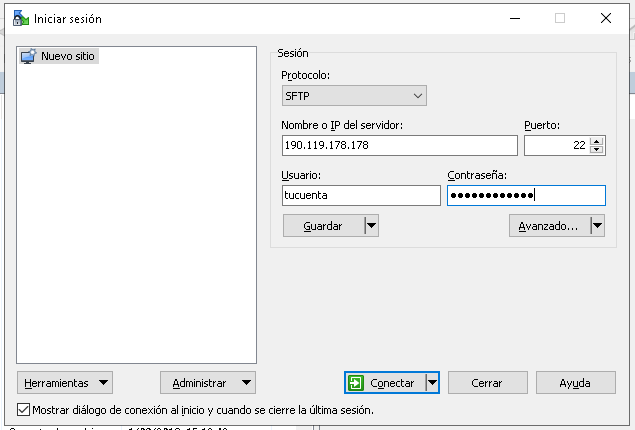
\includegraphics[width=12.4cm]{winscp_1}
    \caption{Interfaz inicial del programa WinSCP}
    \label{fig:winscp_1}
\end{figure}

Al pulsar el botón conectar (luego de rellenar los campos requeridos), será necesario que se acepte la advertencia mostrada en la figura \ref{fig:winscp_alerta}.

\begin{figure}[!ht]
    \centering
    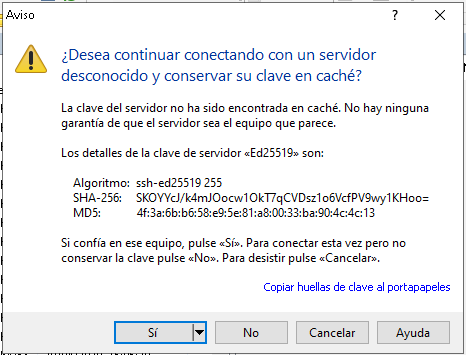
\includegraphics[width=6.4cm]{winscp_alerta}
    \caption{Alerta mostrada por WinSCP, que solicita agregar el host como una fuente confiable}
    \label{fig:winscp_alerta}
\end{figure}

Una vez aceptada dicha advertencia, WinSCP nos mostrará la siguiente interfaz, la cual nos permitirá subir y descargar archivos al clúster Inkari.

\begin{figure}[!ht]
    \centering
    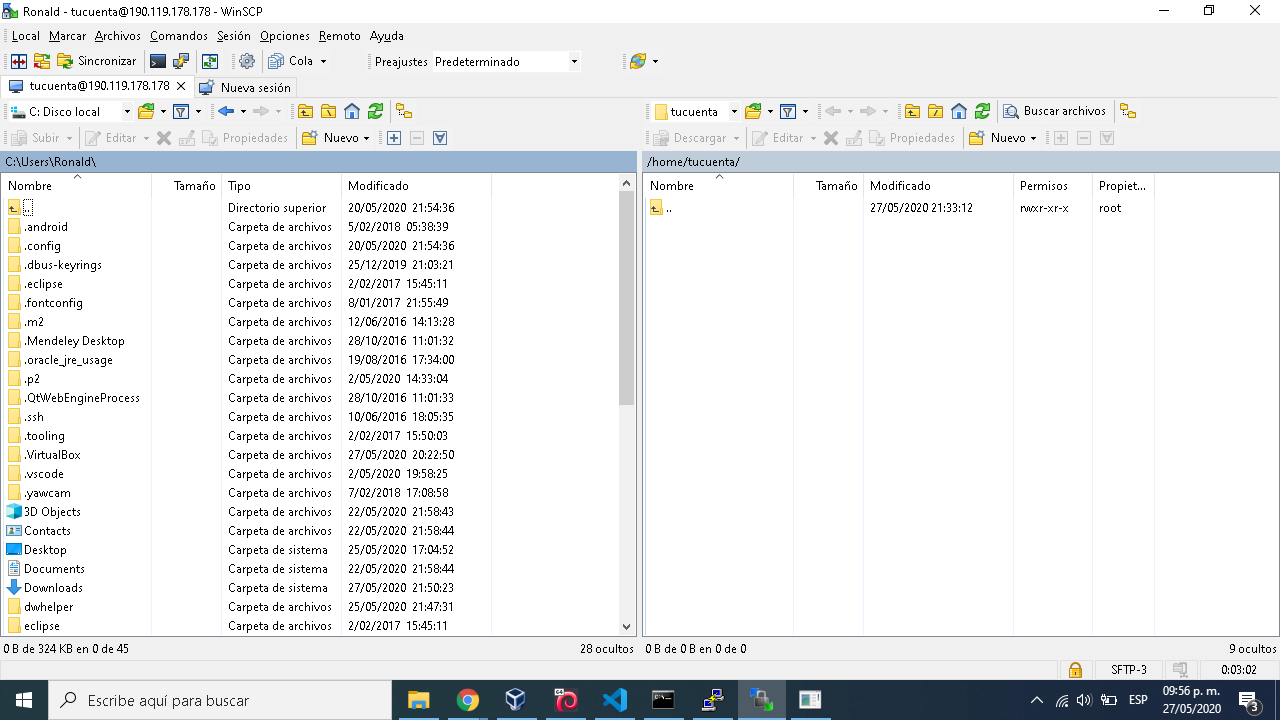
\includegraphics[width=13.7cm]{winscp_conectado}
    \caption{Interfaz de WinSCP, conectado al clúster Inkari}
    \label{fig:winscp_conectado}
\end{figure}

\newpage

Si la conexión se realizó de forma exitosa, ud. deberá de visualizar la interfaz mostrada en la figura \ref{fig:winscp_conectado}.

\section{Revisión de los recursos}

Para revisar si existen recursos disponibles en Inkari, deberemos de usar el comando \textbf{sinfo}, dicho comando nos permitirá visualizar el estado de cada uno de los nodos, en la figura \ref{fig:sinfo} se observa un ejemplo de su salida.

\begin{figure}[!ht]
    \centering
    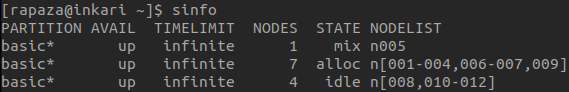
\includegraphics[width=8.2cm]{sinfo}
    \caption{Ejemplo de la salida del comando \textbf{sinfo}}
    \label{fig:sinfo}
\end{figure}

En donde, los estados mostrados significan lo siguiente: 

\begin{table}[!ht]
\centering
\begin{tabular}{|l|l|}
\hline
\multicolumn{1}{|c|}{\textbf{Estado}} & \multicolumn{1}{c|}{\textbf{Significado}} \\ \hline
\textbf{ALLOC} & Indica que el nodo está siendo usado en toda su capacidad. \\ \hline
\textbf{MIX} & \begin{tabular}[c]{@{}l@{}}Indica que el nodo está siendo usado en forma incompleta, \\ quedando recursos para recibir nuevos jobs.\end{tabular} \\ \hline
\textbf{IDLE} & \begin{tabular}[c]{@{}l@{}}Indica que el nodo está absolutamente libre y operativo \\ para recibir nuevos jobs.\end{tabular} \\ \hline
\end{tabular}
\caption{Ejemplo de la salida del comando \textbf{sinfo}}
\label{tab:sinfo}
\end{table}

En caso de que desee visualizar que recursos disponibles en un nodo con estado MIX, se podrá hacer uso del comando \textbf{check-resources}, el cual nos mostrará un listado de todos los nodos con la cantidad de cpus y memoria disponible; y que cantidad de estos esta siendo utilizada (esto puede observarse en la figura \ref{fig:check}.

\begin{figure}[!ht]
    \centering
    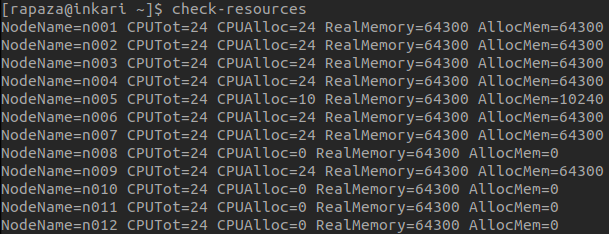
\includegraphics[width=12.2cm]{check}
    \caption{Ejemplo de la salida del comando \textbf{check-resources}}
    \label{fig:check}
\end{figure}

\section{Uso de librerías}

Para poder observar el listado de los softwares (módulos) disponibles se debe de ejecutar el siguiente comando:

\begin{lstlisting}
    module avail
\end{lstlisting}

Un ejemplo de la ejecución del comando es mostrado a continuación:

\begin{figure}[!ht]
    \centering
    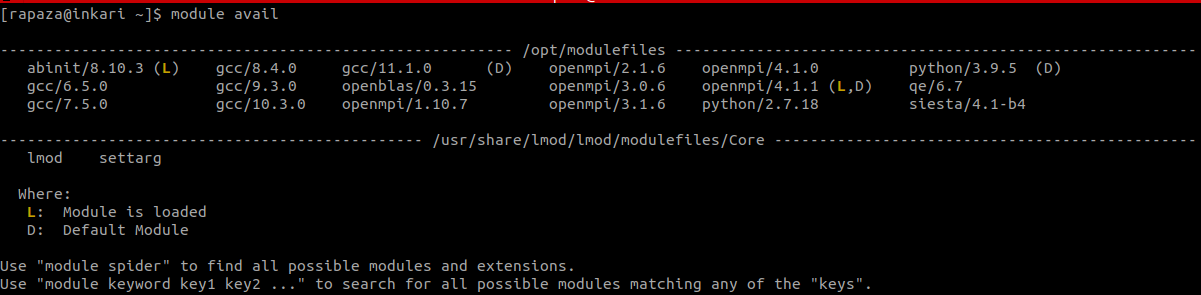
\includegraphics[width=14cm]{module_avail}
    \caption{Salida de la ejecución del comando module avail}
    \label{fig:module_avail}
\end{figure}

\begin{note}
    Las librerías listadas en la figura \ref{fig:module_avail}, pueden variar con el paso del tiempo.
\end{note}

Si deseamos utilizar una librería, deberemos ejecutar el comando: \textit{module load } y luego el nombre de la librería tal y como aparece en el listado de \textit{module avail}, por ejemplo, si deseamos hacer uso de la librería abinit 8.10.3, deberemos de ejecutar el siguiente comando:

\begin{lstlisting}
    module load abinit/8.10.3
\end{lstlisting}

\begin{note}
    También es posible utilizar solo el nombre de la librería (\textit{module load abinit}), sin embargo esto cargará la versión que tiene por defecto dicha librería y en este caso será la 8.10.3 por ser la única disponible.
\end{note}

Finalmente se resalta que al momento de cargar una librería, esta cargará todas las dependencias necesarias, por ejemplo si cargamos la librería abinit y posteriormente ejecutamos el comando: \textit{module list} se observa que también ya se cargo la librería OpenMPI 4.1.1.

\begin{figure}[!ht]
    \centering
    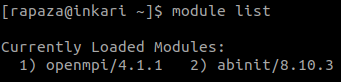
\includegraphics[width=6cm]{module_list}
    \caption{Listado de módulos cargados, tras cargar únicamente abinit}
    \label{fig:module_list}
\end{figure}

\begin{note}
    Algunos ejemplos del uso de las librerías instaladas se encuentran en el github de inkari, para acceder a ellos ingrese a: \url{https://github.com/unsa-inkari}.
\end{note}

\section{Envío de trabajos}

El envío de trabajos al clúster Inkari se realiza mediante el gestor de colas SLURM.
Para enviar un trabajo al clúster, primero se tendrá que almacenar los archivos necesarios en la supercomputadora y luego solo se deberá de ejecutar el siguiente comando:

\begin{lstlisting}
    sbatch script.slrm
\end{lstlisting}

El comando sbatch y el contenido del script (script.slrm) permiten especificar ciertos flags (parámetros) que se tendrán en cuenta al momento de ejecutar el trabajo, por ejemplo, si se desea asignar un nombre específico a nuestro trabajo, se tendría que utilizar el siguiente comando:

\begin{lstlisting}
    sbatch script.slrm --job-name <nombre_del_trabajo>
\end{lstlisting}

También es posible asignar dichos flags al contenido de nuestro script, para ello se utiliza la siguiente sintaxis:

\begin{center}
    \#SLURM \texttt{-{}-}job-name <nombre\_del\_trabajo>
\end{center}

\newpage

A continuación se describen algunos de los flags usualmente utilizados:

\begin{table}[!ht]
\centering
\begin{tabular}{|l|l|l|}
\hline
\multicolumn{1}{|c|}{\textbf{Opción}} & \multicolumn{1}{c|}{\textbf{Ejemplo de valor}} & \multicolumn{1}{c|}{\textbf{Descripción}} \\ \hline
\texttt{-{}-}job-name & nombre-del-job & \begin{tabular}[c]{@{}l@{}}Permite asignar un nombre al\\ job\end{tabular} \\ \hline
\texttt{-{}-}nodelist & n006,n009,n011 & \begin{tabular}[c]{@{}l@{}}Indica una lista de nodos en\\ los que se deberá de ejecutar\\ el job\end{tabular} \\ \hline
\texttt{-{}-}nodes & 1 & \begin{tabular}[c]{@{}l@{}}Usado para asignar la\\ cantidad de nodos a utilizar\end{tabular} \\ \hline
\texttt{-{}-}ntasks-per-node & 12 & \begin{tabular}[c]{@{}l@{}}Usado para asignar el\\ número de tareas por nodo\end{tabular} \\ \hline
\texttt{-{}-}mem-per-cpu & 2G & \begin{tabular}[c]{@{}l@{}}Indica la cantidad de\\ memoria que usará cada\\ cpu\end{tabular} \\ \hline
\texttt{-{}-}mem & 24G & \begin{tabular}[c]{@{}l@{}}Indica la cantidad de\\ memoria que usará todo el\\ job\end{tabular} \\ \hline
\texttt{-{}-}output & output\texttt{-}\%j.out & \begin{tabular}[c]{@{}l@{}}Usado para establecer el\\ nombre del archivo de la\\ salida estándar\end{tabular} \\ \hline
\texttt{-{}-}error & output\texttt{-}\%j.err & \begin{tabular}[c]{@{}l@{}}Usado para establecer el\\ nombre del archivo de la\\ salida de error\end{tabular} \\ \hline
\texttt{-{}-}time & 720:00:00 & \begin{tabular}[c]{@{}l@{}}Utilizado para asignar el\\ tiempo máximo de ejecución\\ del job\end{tabular} \\ \hline
\end{tabular}
\caption{Listado de opciones pra el envío de jobs}
\label{tab:params}
\end{table}

Para profundizar en los flags que pueden ser utilizados, se recomienda la lectura de la siguiente web: \url{https://slurm.schedmd.com/sbatch.html}.

\begin{note}
    Si desea ver un script básico que hace uso de las opciones anteriormente mencionadas, ingrese a: \url{https://github.com/unsa-inkari/template-basic}.
\end{note}

\newpage

\section{Monitorización de jobs}

Para monitorear los trabajos enviados se puede usar el comando \textit{squeue}, un ejemplo de su uso es mostrado a continuación.

\begin{lstlisting}
    squeue -l
\end{lstlisting}

La ejecución de este comando con la bandera \textbf{l} proporciona una mayor información, tales como: el identificador del trabajo (columna 1), el nombre del trabajo (columna 3), el estado del trabajo (columna 5), entre otros, un ejemplo de esto puede verse en: \ref{fig:squeuel}.

\begin{figure}[!ht]
    \centering
    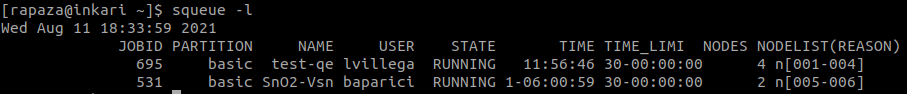
\includegraphics[width=12cm]{squeuel}
    \caption{Monitorización de trabajos enviados, mediante el comando squeue}
    \label{fig:squeuel}
\end{figure}

\section{Detención de la ejecución de jobs}

Finalmente, en el caso de que se desee cancelar un trabajo enviado, se debe de utilizar el siguiente comando: 

\begin{lstlisting}
    scancel <identificador_del_trabajo>
\end{lstlisting}

\end{document}
